\input ../SlidePreamble
\input ../preamble


\begin{document}

{\Huge


\centerline{\bf TTIC 31230, Fundamentals of Deep Learning}
\bigskip
\centerline{David McAllester, Winter 2020}

\vfill
\centerline{\bf Double Descent}
\vfill
\vfill
\vfill

\slide{Double Descent}

{\huge
Reconciling modern machine learning practice and the bias-variance trade-off

\bigskip
Mikhail Belkin, Daniel Hsu, Siyuan Ma, Soumik Mandal, arXiv December 2018.

\vfill
Deep Double Descent: Where Bigger Models and More Data Hurt

\bigskip
Preetum Nakkiran, Gal Kaplun, Yamini Bansal, Tristan Yang, Boaz Barak, Ilya Sutskever, ICLR 2020
}

\slide{Double Descent}

\centerline{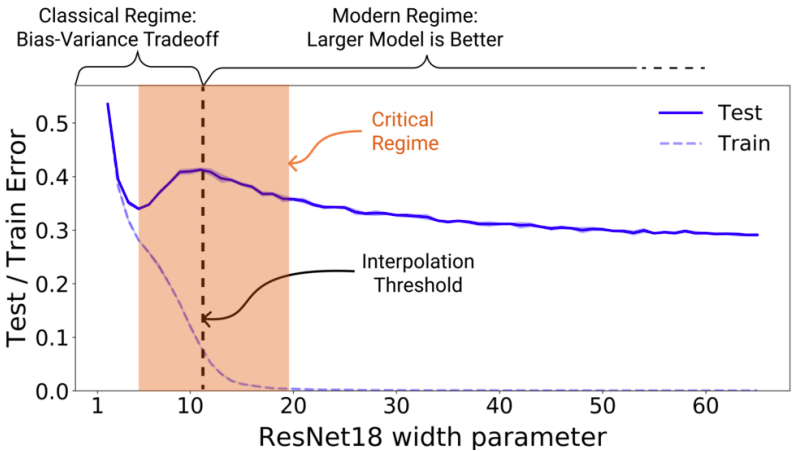
\includegraphics[width = 6in]{\images/DoubleDescent1}}

\vfill
Deep Double Descent: Where Bigger Models and More Data Hurt

\bigskip
Preetum Nakkiran, Gal Kaplun, Yamini Bansal, Tristan Yang, Boaz Barak, Ilya Sutskever, ICLR 2020

\slide{Double Descent}

\centerline{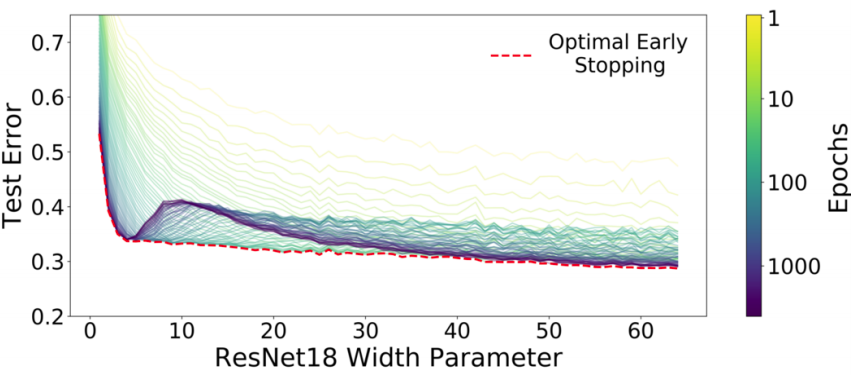
\includegraphics[width = 8in]{\images/DoubleDescent2}}

\slide{Summary}

There is never harm in doing early stopping --- one should always do early stopping.

\vfill
Regularization is any modification to the training algorithm motivated by reducing the training-validation gap.

\vfill
While regularization modifications to training can be inspired by theory, the theory is weak.

\vfill
Regularization proposals should be evaluated empirically.

\slide{END}

}
\end{document}
